%!TEX root = /lecture/Discrete_Optimistic.tex

\paragraph{Analysis}
\[\begin{aligned}
    \Ebb[\text{cut value}]&=\sum_{(i,j)\in E}\omega(i,j)\cdot\mathrm{Pr}[(i,j)\text{ cut}]\\
    &=\sum_{(i,j)\in E}\omega_{ij}\cdot\frac{\arccos\<v_i,v_j\>}{\pi}\\
    & \geq \alpha_{GW}\sum_{(i,j)\in E}\omega_{ij}\cdot\frac{1-\<v_i,v_j\>}{2}
\end{aligned}\]
where 
\[\alpha_{GW}=\inf_{\rho\in[-1,1]}\frac{\frac{1}{\pi}\arccos\rho}{\frac{1}{2}(1-\rho)}\approx 0.87856\]

\paragraph{Integrality Gap}

$ 5 $-Cycle:

\begin{center}
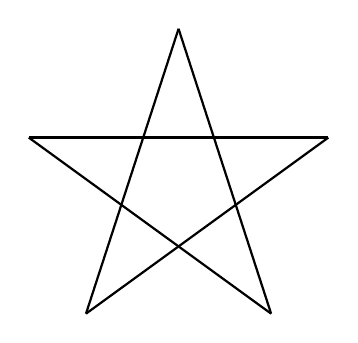
\begin{tikzpicture}% pentagon
    \draw[thick] (90:2) -- (234:2);
    \draw[thick] (234:2) -- (18:2);
    \draw[thick] (18:2) -- (162:2);
    \draw[thick] (162:2) -- (306:2);
    \draw[thick] (306:2) -- (90:2);
\end{tikzpicture}
\end{center}

Then  $ \OPT=4/5 $, 
\[\mathrm{SDP} \geq \frac{1-\cos 144^\circ}{2}\approx 0.9045\]
Gap ratio  $  \leq \frac{0.8}{0.9045}\approx 0.885 $.

\paragraph{Embedded graph}  $ G=(V,E, \omega) $, consider  $ V\subset S^{d-1}=\{\|x\|^2=1\} $.
\[\mathrm{Obj}(G)=\sum_{(\vec{x},\vec{y})\in E}\omega(\vec{x},\vec{y})\frac{1-\<\vec{x},\vec{y}\>}{2}\]
\begin{fact}
    $ \forall  $ embedded graph  $ G $,  $ \mathrm{SDP(G)} \geq \mathrm{Obj}(G) $. 
\end{fact}  

\paragraph{Gap Instance}  $G_d=(V,E), V=S^{d-1},E=V\times V $.

Let  $ \omega(\vec{x},\vec{y}) $ be the probability density of 
\[\vec{x}\sim S^{d-1},y\sim S^{d-1}|\<\vec{x},\vec{y}\> \leq \rho^*\]
Clearly, for this infinite graph,  $ \mathrm{SDP}(G) \geq \mathrm{Obj}(G) \geq \frac{1-\rho^*}{2} $. 

For  $ A\subset S^{d-1}$, 
\[\mu_l(A)=\mathrm{Pr}_{\vec{x},\vec{y}\sim S^{d-1}}\left[\vec{x}\in A\oplus \vec{y}\in A\left|\<\vec{x},\vec{y}\> \leq \rho\right.\right]\] 
\begin{theorem}
    For  $ \forall a\in [0,1],\rho\in [-1,1] $,  $ \max_{A:\text{ measure of  $ A=a $ }}\{\mu_{\rho}(A)\} $ is achieved when  $ A  $ is a cap of  $ S^d $.   
\end{theorem}
\begin{corollary}
     $ \max\{\mu_{\rho^*}(A)\} $ is achieved when measure of  $ A=\frac{1}{2} $.   
\end{corollary}
\begin{claim}
    \[\OPT(G_d) \leq \frac{\arccos \rho^*}{\pi}+O(\frac{1}{\sqrt{d}}) \]
\end{claim}
Leave as a homework.

Assume Unique Game Conjecture,  $ \alpha_{GW} $ is the best Integrality Gap.

\paragraph{Algorithmic Gap}
\begin{example}[Instance]
    $ H_d=(V,E,\omega) $,  $ \dps V=\{\pm\frac{1}{\sqrt{d}}\}^d $.  $ \omega\sim  $ distribution,  $ \vec{x}\sim V $, 
    \begin{equation}
        y_i=\begin{cases}
            x_i&\text{ with prob } \frac{1+\rho^*}{2}\\
            -x_i&\text{ with prob } \frac{1-\rho^*}{2}
        \end{cases}\label{def: sim_rho}
    \end{equation}
    denoted as  $ \vec{y}\sim_{\rho^*}\vec{x} $.
    
    Then  $ \Ebb x_i=\Ebb y_i=0 $,  $ \Ebb x_iy_i=\left(\frac{1+\rho^*}{2}\right)\cdot 1+\left(\frac{1-\rho^*}{2}\right)(-1)=\rho^* $.
\end{example}

\begin{fact}
    \[ \mathrm{Obj}(H_d)=\Ebb_{(\vec{x},\vec{y})\sim \omega}\left[\frac{1-\<\vec{x},\vec{y}\>}{2}\right]=\frac{1}{2}-\frac{1}{2}\rho^* \]
    \[\mathrm{SDP} \geq \frac{1}{2}-\frac{1}{2}\rho^*\]
\end{fact}
\begin{claim}\label{claim: sdp_gap}
    \[\mathrm{SDP} \leq \frac{1}{2}-\frac{1}{2}\rho^*\]
\end{claim}
By the claim, 
\[\Ebb[\text{rounding}]=\Ebb_{(\vec{x},\vec{y})\sim \omega}\frac{\arccos\<\vec{x},\vec{y}\>}{\pi} \leq \frac{\arccos\rho^*}{\pi}+O(\frac{1}{\sqrt{d}})\]
\[\OPT=\frac{1}{2}-\frac{1}{2}\rho^*\]

\paragraph{Fourier Analysis of Boolean Function}
Boolean function:  $ f:\{\pm 1\}^n\rightarrow \Rbb $.

Inner product  $ \<f,g\>=\Ebb_{\vec{x}\sim \{\pm 1\}^n}[f(x)\cdot g(x)] $ 

\textit{Fourier basis}  

$ \forall s\subset [n] $,  $ \chi_s(x)=\dps\prod_{i\in s}x_i $  

$ \<\chi_s,\chi_s\>=\Ebb_{\vec{x}}\chi_s^2(x)=1 $.

$ \dps\forall s\neq t, \,\<\chi_s,\chi_t\>=\Ebb_{\vec{x}}\chi_s(\vec{x})\cdot\chi_t(\vec{x})=\Ebb_{\vec{x}}\chi_{s\Delta t}(\vec{x})=\prod_{i\in s\Delta t}\Ebb[x_i]=0 $.

So  $ \{\chi_s\} $ forms an orthonormal basis.

\begin{proposition}[Fourier expansion]
    $ \forall f:\{\pm 1\}^n\rightarrow \Rbb $, 
    \[f=\sum_{s\subset [n]}\hat{f}(s)\cdot\chi_s\] 
    where  $ \hat{f}(s)=\<f,\chi_s\> $. 
\end{proposition}

\begin{theorem}[Parseval's]
    $ \forall f: \{\pm 1\}^n\rightarrow \{\pm 1\}$,
    \[\sum_{s\subset [n]}\hat{f}(s)^2=\<f,f\>=1\] 
\end{theorem}
\paragraph{Noise Stability}
 $ f:\{\pm 1\}^n\rightarrow \{\pm 1 \} $.
 \[\mathrm{NS}_\rho(f)=\mathrm{Pr}_{\vec{x},\vec{y}\sim_\rho \vec{x}}[f(\vec{x})=f(\vec{y})]\]
Recall the notation of  $ \sim_\rho $ in  \eqref{def: sim_rho}.

\[\begin{aligned}
    \mathrm{NS}_\rho(f)&=\mathrm{Pr}_{\vec{x},\vec{y}\sim_\rho \vec{x}}[f(\vec{x})=f(\vec{y})]\\
    &=\Ebb_{\vec{x},\vec{y}\sim_\rho \vec{x}}\frac{1+f(\vec{x})f(\vec{y})}{2}\\
    &=\frac{1}{2}+\frac{1}{2}\Ebb_{\vec{x},\vec{y}\sim_\rho\vec{x}}f(\vec{x})\cdot f(\vec{y})
\end{aligned}\]
\[\begin{aligned}
    &\quad\Ebb_{\vec{x},\vec{y}\sim_\rho\vec{x}}\left(\sum_{s}\hat{f}(s)\chi_s(x)\right)\left(\sum_t\hat{f}(t)\chi_t(\vec{y})\right)\\
    &=\sum_{s,t}\hat{f}(s)\hat{f}(t)\Ebb_{\vec{x},\vec{y}\sim_\rho\vec{x}}\chi_s(\vec{x})\chi_t(\vec{y})\\
    &=\sum_{s,t}\hat{f}(s)\hat{f}(t)\Ebb_{\vec{x}}\chi_s(\vec{x})\chi_t(\vec{x})\cdot\Ebb_{\vec{u}}\chi_t(\vec{\mu})\qquad\text{where  $ \vec{y}=\vec{x}\cdot \vec{\mu} $}\\
    &=\sum_{s,t}\hat{f}(s)^2\cdot\rho^{|s|}
\end{aligned}\]
So 
\[\mathrm{NS}_\rho(f)=\frac{1}{2}+\frac{1}{2}\sum_s\hat{f}(s)^2\cdot \rho^{|s|}\]